\section{Clock \& Reset}

The mmRISC-1 has two clock domains; one is CLK (System Clock) and the other is TCK (JTAG Clock). These clocks are asynchronous, so clock domain crossing logic is used in DTM (Debug Transport Module).\\
The Reset Structure of mmRISC-1 is slightly  complicated as shown in Figure\ref{fig:RESET}. RES\_ORG is the origin of chip reset such as power-on-reset or reset from external pin. RES\_DBG, which is controlled by DTMCS, is a reset signal only for debug logic.  DMCONTROL can control both RES\_SYS and HART\_RESET[ ] . RES\_SYS is a system reset for the whole chip and peripherals. HART\_RESET[ ] are connected to each CPU (Hart) and can independently reset each hart. In each CPU (Hart), one of the HART\_RESET signals is renamed to RES\_CPU, and the RES\_CPU resets the whole area in the CPU block. In the chip top layer, SRSTn is a bi-directional inout signal. The SRSTn input is used to reset the whole chip except for the debug block, and the SRSTn output is generated from the debug block.\\

\begin{figure}[H]
    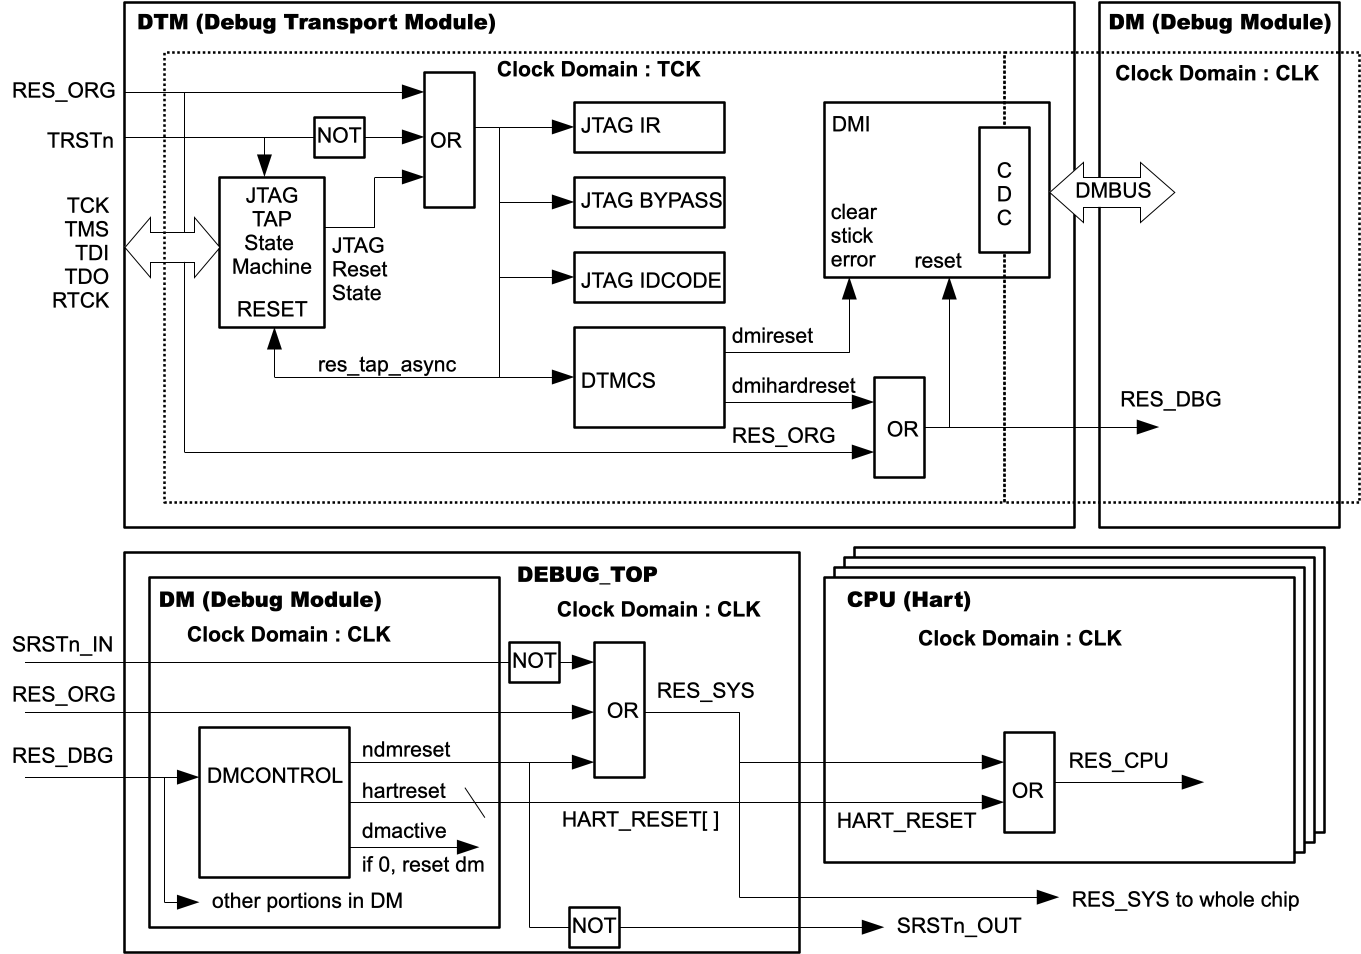
\includegraphics[width=1.00\columnwidth]{./Figure/Reset.png}
    \caption{Reset Structure}
    \label{fig:RESET}
\end{figure}

